%!TEX program = xelatex
\documentclass[cn,hazy,blue,10.5pt,normal]{elegantnote}
\title{Nas Server:个人云服务搭建过程}

\author{clay}
\institute{\LaTeX{} Program}

\version{1.0}
\date{\zhtoday}

\usepackage{array}
\usepackage{caption}
\usepackage{hyperref}
\usepackage{url}

\begin{document}

\maketitle

\centerline{
  
\includegraphics[scale=0.2]{head.jpg}
}

\newpage
\section{Nas Server 硬件设备}

\begin{itemize}
  \item 树莓派4B 2G内存版 $\rightarrow$ 软路由
  \item 红米路由器 AX3000 $\rightarrow$ 路由器
  \item ASUS笔记本 $\rightarrow$ Nas Server
  \item 一条拥有公网ip的电信宽带
  \item 一条swjtu校园宽带
\end{itemize}

\begin{figure}[!htb]
  \centering
  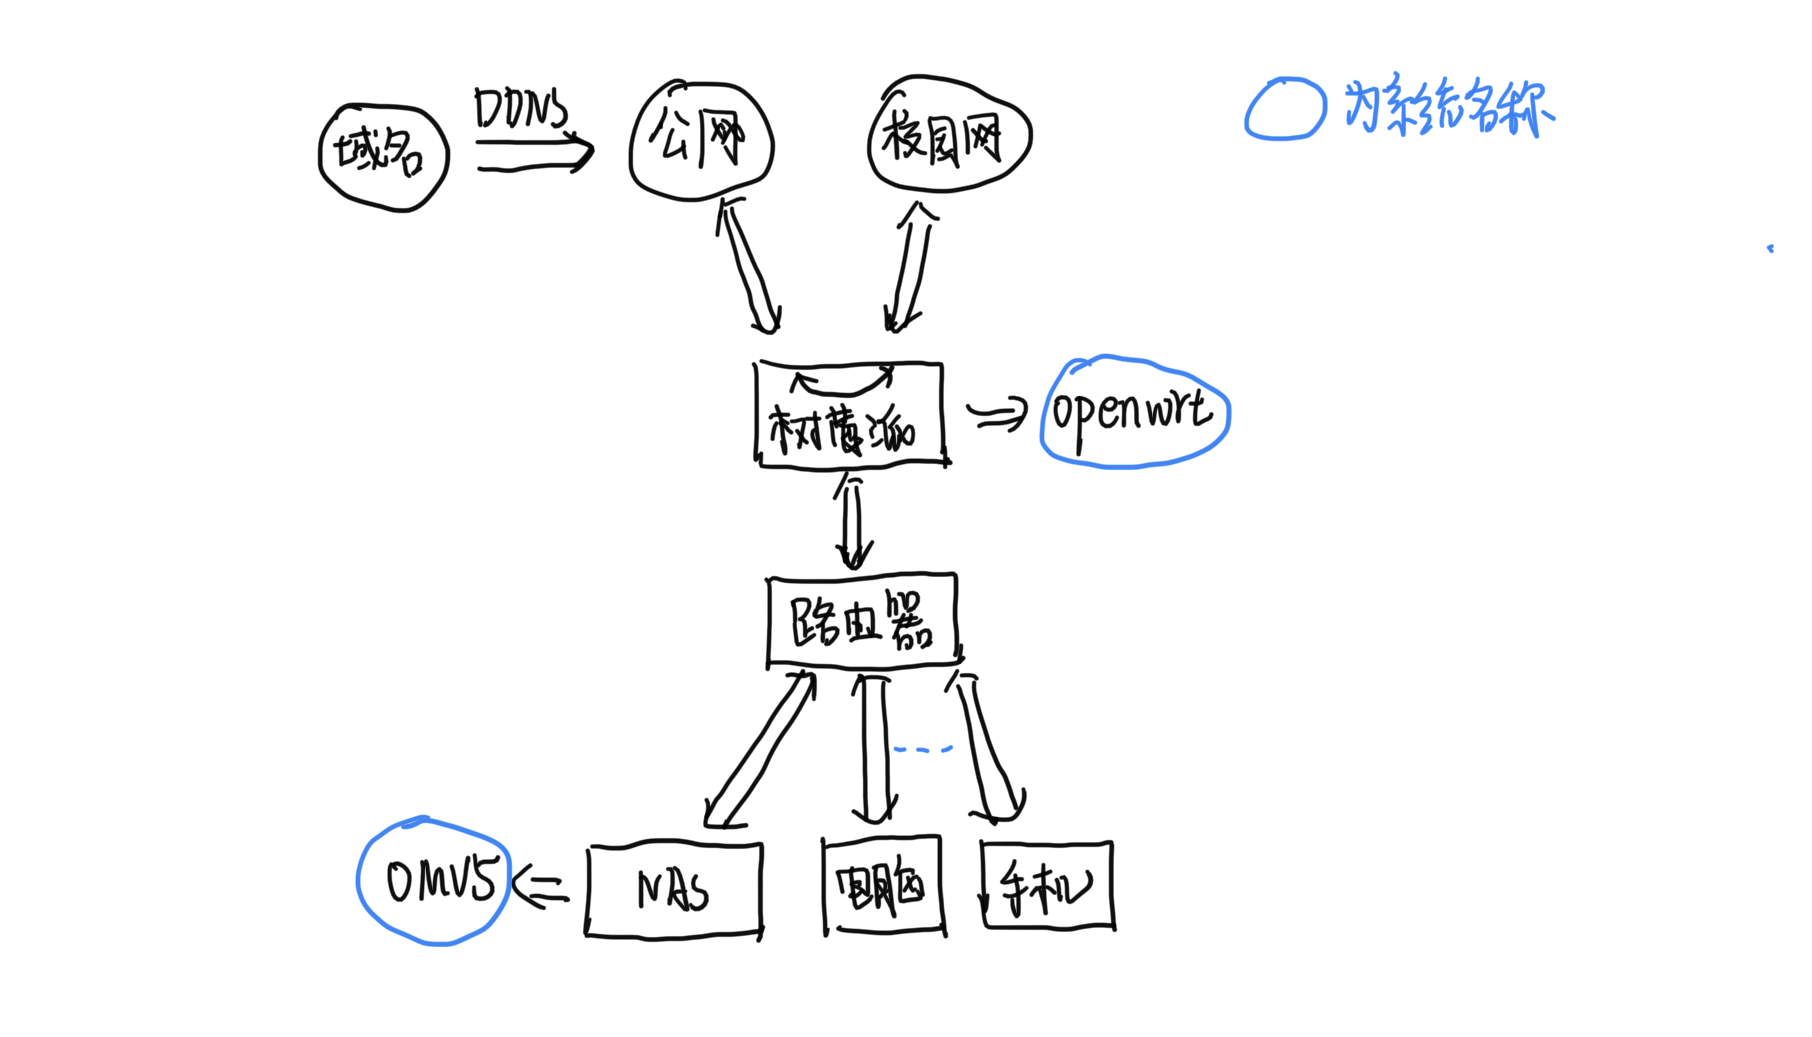
\includegraphics[scale=0.25]{image/系统架构.PNG}
  \caption{整体系统框架}
\end{figure}

\subsection{软路由}

在Nas Server中,软路由作为系统的网络的交通枢纽,使用的是OpenWrt系统基于Linux系统。作为系统的网络交通枢纽,树莓派在其中做的事情有,通过对公网和校园网拨号连接网络,通过lan口连接下级路由器分享网络。除了基础的网络功能外,还使用了DDNS功能、OpenClash、负载均衡和端口转发等功能。

\subsubsection{OpenWrt网络结构}

Openwrt 网络结构框架

\begin{figure}[htbp]
  \centering
  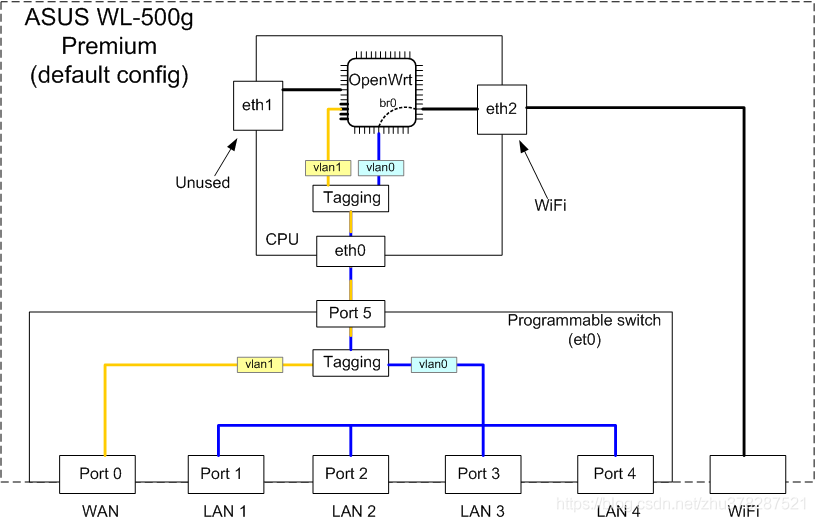
\includegraphics[scale=0.45]{image/OpenWrt.png}
  \small
  \caption{Openwort 网络结构框架}\label{fig:1.1}
\end{figure}

在本项目中,我的方案是把公网和校园网划分为

\newpage

OpenWrt 网络端口分配

\begin{figure}[!htb]
  \centering
  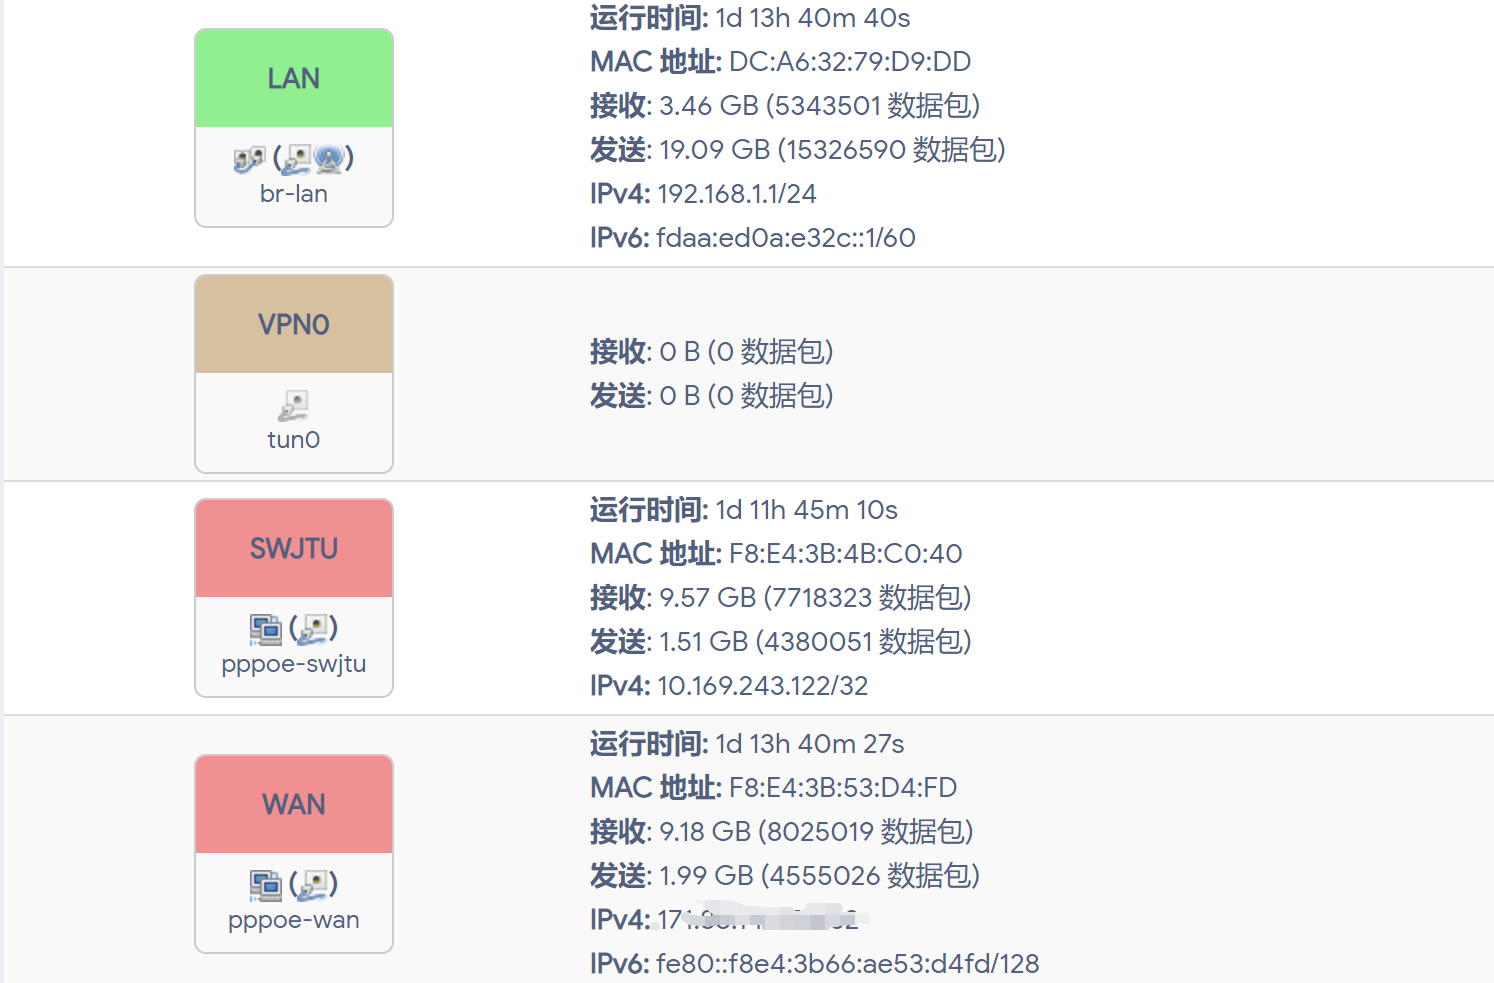
\includegraphics[scale=0.25]{image/port.png}
  \caption{Openwort 网络接口分配}\label{fig:1.2}
\end{figure}

\subsubsection{资源下载}
树莓派4B如何安装OpenWrt软路由:\url{https://www.bilibili.com/read/cv9714518}


树莓派4B所需OpenWrt镜像源下载链接:\url{https://pan.baidu.com/s/166mxMyDtEPjf5OGO7mchwA}  提取码:ewlk 


U盘镜像烧录软件下载连接:\url{https://pan.baidu.com/s/1ZE-2NpENZL9sGLu9RALqPQ}  提取码:fw5b


\subsubsection{问题总结} 

\textbf{已解决问题}
\begin{itemize}
  \item 在刚开始配置软路由时,OpenWrt管理界面无法进入,原因为刚开始配置时不能插网线,等通过wifi设置网口pppoe通信时,插入网线即可实现拨号。
  \item 使用OpenWrt系统的过程中,当没有配置网口的通信方式时,直接插网口会导致一开始配置的网口出现问题
  \item 负载均衡中的源地址和目的地址理解性错误,源地址统指客户端即本地的pc端,目的地址为客户端要到达的地址
  \item 无法访问实验室服务器问题,在静态路由中添加路由表解决。
  \item DDNS配置问题,可以查看文件\href{run:./other_guide/openwrt_set_DDNS.pdf}{DDNS}
  \item 公网无法访问路由器下的Nas设备,解决功能通过防火请的端口转发功能。
\end{itemize}

\textbf{未解决问题}
\begin{itemize}
  \item Wifi情况下王者荣耀能够登录但是无法对战情况。
  \item 并不能够实现单线多拨,或者多线多拨的功能。
  \item 
\end{itemize}

\textbf{未来计划}
\begin{itemize}
  \item 当检测到公网ip发生变化时,通过邮件等方式通知用户。(已实现,代码链接\url{https://github.com/guoclay/interesting-project/tree/master/Nas%20Server/send_ip})
  \item 建立交互式界面,能够对校园网内电脑进行交互式访问。
\end{itemize}



\subsection{路由器}
路由器在系统中起到的作用并不大,主要的作用有对软路由进行端口转发,产生wifi信号等。

\subsection{Nas Server}



\end{document}
